\chapter{$M_{\rm BH} - L_{\rm gal}$, $M_{\rm BH} - L_{\rm sph}$ and $M_{\rm BH} - M_{\rm *,sph}$ }
\label{ch:mm} 

In Chapter \ref{ch:galviv}, reliable and accurate multicomponent decompositions were presented 
for 66 galaxies, our final sample, out of the 75 belonging to the initial sample. 
These 66 galaxies currently constitute the largest sample to date 
with reliable and homogeneous (i.e.~derived in a systematic and consistent manner) 
structural decompositions 
that can be used to investigate correlations between 
directly measured black hole masses and host galaxy parameters. \\

This Chapter is dedicated to the analysis of three black hole mass correlations: 
the $M_{\rm BH} - L_{\rm gal}$, $M_{\rm BH} - L_{\rm sph}$ and $M_{\rm BH} - M_{\rm *,sph}$ relations. 
Four principal questions will be addressed. 

\begin{enumerate}

\item Is the $M_{\rm BH} - L_{\rm sph}$ relation more fundamental than the $M_{\rm BH} - L_{\rm gal}$ relation 
      (e.g.~\citealt{kormendyho2013}), 
      or are they equally important (e.g.~\citealt{lasker2014anal})?

\item \cite{grahamscott2013} identified two different sequences of spheroids in the $M_{\rm BH} - L_{\rm sph}$ 
      diagram, namely S\'ersic and core-S\'ersic. 
      However, their bulge luminosities were not derived from individual galaxy decompositions, 
      but they were inferred from observed, total galaxy magnitudes 
      through a mean statistical correction. 
      Do we recover their result here, using the present dataset? 
           
\item Does the quality of the present dataset allow us to identify any (additional) substructure 
      in the three diagrams under study?
       
\item Some studies have distinguished pseudo-bulges and classical bulges according to their S\'ersic index, 
      and claimed that in the $M_{\rm BH} - L_{\rm sph}$ diagram 
      pseudo-bulges are offset from the correlation defined by classical bulges. 
      Here we test this result with our data. 

\end{enumerate}

A robust linear regression analysis is crucial for the study of black hole mass correlations.
In particular, more emphasis is typically given to the slope rather than the intercept of scaling relations, 
because the slope is the parameter that theoretical models (currently) 
predict\footnote{However, more and more attention is being paid to the intercept of black hole mass scaling relations, 
which plays a major role for the prediction of cosmic gravitational waves background from SMBH binary coalescence 
(e.g.~\citealt{shannon2015,shankar2016}), 
the derivation of the SMBH mass function and space density, 
or the calibration of the reverberation mapping virial factor. }. 
Several studies (e.g.~\citealt{tremaine2002,graham2007,tundo2007,graham2016review}) 
have pointed out inconsistencies between the values of the slope
measured by different groups for the same correlation. 
These discrepancies can arise from the use of different galaxy samples, 
selection biases, or the statistical techniques used to perform the linear regression analysis. \\

In the following analysis, we will make use of three linear regression routines: 
the {\tt BCES} code from \cite{akritasbershady1996}, 
the {\tt FITEXY} routine \citep{press1992}, as modified by \cite{tremaine2002}, 
and the Bayesian estimator {\tt linmix\_err} \citep{linmixerr}.
Albeit its remarkable computational speed, 
the {\tt BCES} estimator is not reliable in case of poor number statistics of the galaxy sample analysed, 
or when at least one low-precision measurement is included in the dataset, 
or if the mean square of the uncertainties associated with the independent variable is comparable to 
the variance of the distribution of the independent variable \citep{tremaine2002}. 
When any of these circumstances occur, 
the modified {\tt FITEXY} routine and the Bayesian estimator {\tt linmix\_err} 
perform better than the {\tt BCES} routine \citep{tremaine2002,novak2006,park2012}. 
All of these three estimators take into account the intrinsic scatter of a correlation, 
but only the {\tt FITEXY} and the {\tt linmix\_err} codes allow one to measure it. 
The interest in measuring the intrinsic scatter of black hole mass scaling relations 
relies on the assumption that 
the galaxy parameter associated with the smallest intrinsic residual variance 
has the best chance of being causally correlated to the black hole mass. \\

The remainder of this Chapter comprises the published version of the paper 
``Supermassive Black Holes and Their Host Spheroids. 
II. The Red and Blue Sequence in the $M_{\rm BH} - M_{\rm *,sph}$ Diagram'' 
by G.~A.~D.~Savorgnan et al.,  
as it appears in Volume 817 of the \emph{The Astrophysical Journal}. 

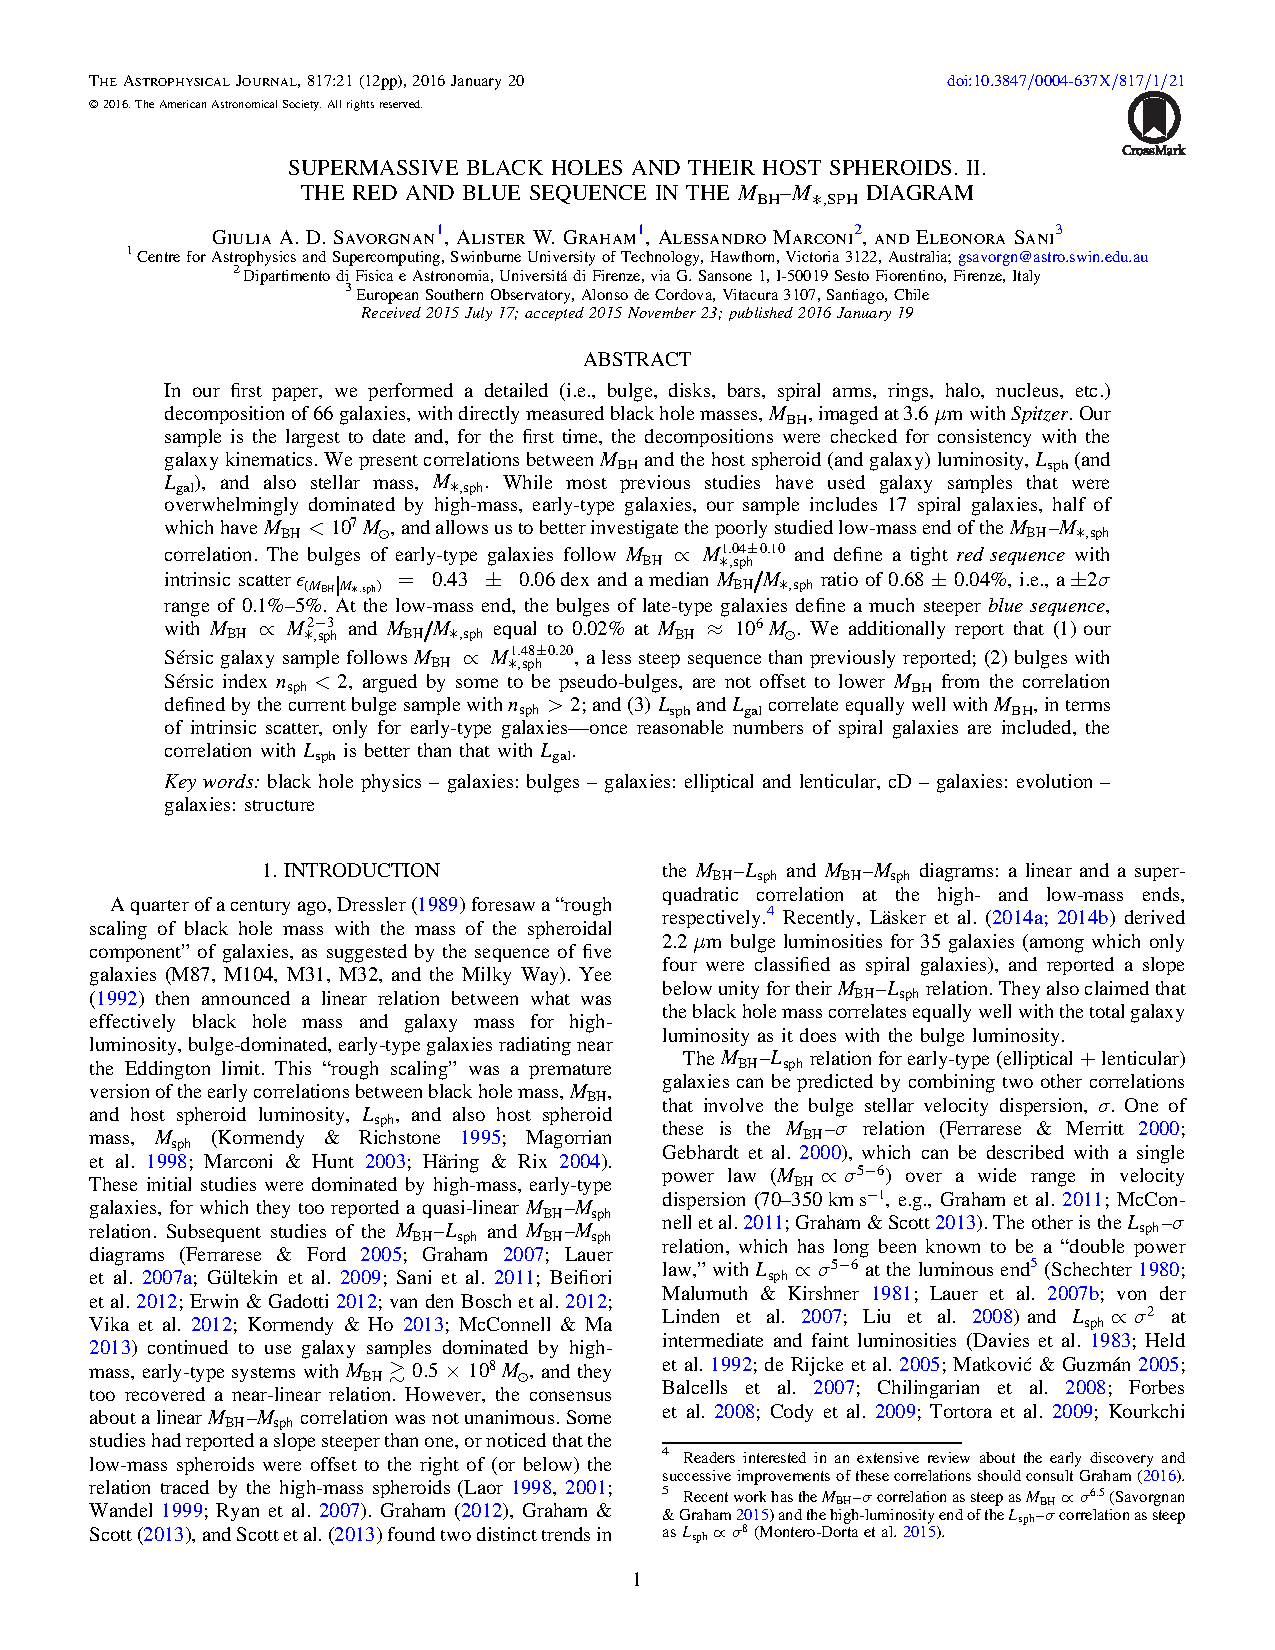
\includepdf[pages={1-12}]{ApJ2016a.pdf}
